\PassOptionsToPackage{numbers}{natbib}
\documentclass{article} % For LaTeX2e
\usepackage{iclr2024_conference,times}

\usepackage[utf8]{inputenc} % allow utf-8 input
\usepackage[T1]{fontenc}    % use 8-bit T1 fonts
\usepackage{hyperref}       % hyperlinks
\usepackage{url}            % simple URL typesetting
\usepackage{booktabs}       % professional-quality tables
\usepackage{amsfonts}       % blackboard math symbols
\usepackage{nicefrac}       % compact symbols for 1/2, etc.
\usepackage{microtype}      % microtypography
\usepackage{titletoc}

\usepackage{subcaption}
\usepackage{graphicx}
\usepackage{amsmath}
\usepackage{multirow}
\usepackage{color}
\usepackage{colortbl}
\usepackage{cleveref}
\usepackage{algorithm}
\usepackage{algorithmicx}
\usepackage{algpseudocode}
\usepackage{tikz}
\usepackage{pgfplots}
\usepackage{float}
\usepackage{array}
\usepackage{tabularx}
\pgfplotsset{compat=newest}


\DeclareMathOperator*{\argmin}{arg\,min}
\DeclareMathOperator*{\argmax}{arg\,max}

\graphicspath{{../}} % To reference your generated figures, see below.

\title{AdaNPC\@: Adaptive Natural-Gradient and Probabilistically-Certified Test-Time Adaptation}

\author{AIRAS}

\newcommand{\fix}{\marginpar{FIX}}
\newcommand{\new}{\marginpar{NEW}}

\begin{document}

\maketitle

\begin{abstract}
We study fully test-time adaptation, where a pretrained model must update itself on an unlabeled stream while respecting strict latency budgets. Popular entropy-minimisation methods such as Tent reduce error on moderate shifts but rely on fixed, source-biased pre-conditioners, assume BatchNorm layers, and can diverge on hard samples. We introduce AdaNPC, a normaliser-agnostic procedure that (i) tracks curvature online with an exponential moving average of squared gradients, (ii) performs a one-shot natural-gradient step pre-conditioned by this Fisher proxy, (iii) safeguards each update with a Bernstein-bound safety filter that rejects steps whose probability of increasing entropy exceeds \(\delta\), and (iv) uses a micro-stepping scheduler to trade accuracy for compute in real time. AdaNPC adapts the affine parameters of Batch, Layer, Group and RMS normalisation layers plus an optional RGB bias, yet adds only a single \(\lvert\theta\rvert\)-sized buffer and \(\leq 5 \%\) extra FLOPs. On ImageNet-C with ResNet-50 it matches the frozen model when Tent, ProxTTA and EATA collapse; on CIFAR-100 it stays stable when the safety filter is disabled; and on a non-stationary ViT stream it degrades gracefully under tight budgets. An ablation confirms the importance of curvature tracking, safety filtering and micro-stepping. The code extends the official Tent repository and requires no hyper-parameter tuning beyond intuitive defaults.
\end{abstract}

\section{Introduction}\label{sec:intro}
Distribution shift between development and deployment is a dominant failure mode of contemporary machine-learning systems. Fully test-time adaptation (TTA) tackles this problem by updating a deployed model on unlabeled test streams, most often by minimising prediction entropy batch-by-batch~\cite{wang-2020-tent}. TTA is attractive because it dispenses with source data, yet four practical obstacles remain.
Curvature drift. Pre-conditioners computed on the source distribution quickly become obsolete as the environment changes, so fixed Fisher or Hessian matrices can mis-scale gradients and harm performance.
Expressiveness. Restricting updates to BatchNorm layers precludes transformer backbones that employ LayerNorm and ignores shifts that affect early filters or input colour.
Safety. Even small unsupervised updates can push the model towards degenerate minima. Existing methods either lack an online certificate of improvement or rely on ad-hoc heuristics that break in dynamic streams~\cite{niu-2023-towards,hoang-2023-persistent}.
Latency. Real-time systems ingest data at a fixed rate; an algorithm that doubles per-batch compute automatically receives only half as many samples to learn from~\cite{alfarra-2023-evaluation}. Thus adaptation must degrade gracefully as compute budgets tighten.
We present AdaNPC---Adaptive Natural-gradient and Probabilistically-Certified TTA---to address all four obstacles simultaneously. AdaNPC maintains a streaming diagonal Fisher proxy and applies a natural-gradient step whose nominal learning rate is one. A Bernstein-style bound estimates the probability that the step would increase entropy; the update is executed only if that probability is \(\leq \delta\). All affine parameters of Batch, Layer, Group and RMS normalisation layers (and optionally a three-parameter RGB bias) are collected into a single vector and updated with identical code. Finally, a micro-stepping scheduler splits the update into \(k\) sub-steps and halves \(k\) whenever the per-batch wall-clock time exceeds a user-specified limit, yielding a smooth accuracy-latency trade-off.
Empirical evaluation covers three scenarios derived from the execution logs. On ImageNet-C with a ResNet-50 backbone AdaNPC tracks the accuracy of the frozen source model while Tent, ProxTTA and EATA collapse. An ablation on CIFAR-100 confirms that disabling the safety filter triggers divergence, whereas removing curvature tracking or micro-stepping yields smaller but measurable losses. A robustness study on a non-stationary ViT stream shows that AdaNPC degrades less sharply than Tent under tight compute budgets, although both harm an already robust transformer.
\subsection{Contributions}
\begin{itemize}
  \item \textbf{Curvature-aware natural gradient}: A natural-gradient step driven by a streaming Fisher proxy that eliminates learning-rate tuning.
  \item \textbf{Probabilistic safety filter}: A closed-form safety certificate that rejects updates likely to increase entropy.
  \item \textbf{Normaliser-agnostic interface}: A unified parameter interface covering BN, LN, GN and RMSNorm layers.
  \item \textbf{Compute-aware micro-stepping}: A scheduler that aligns adaptation cost with real-time budgets.
  \item \textbf{Empirical insights}: A study revealing both strengths (stability, efficiency) and weaknesses (transformer robustness) of AdaNPC\@.
\end{itemize}
Future work will combine AdaNPC with richer unsupervised objectives such as conjugate pseudo-labels~\cite{goyal-2022-test}, extend curvature tracking to transformer attention weights, and incorporate persistence mechanisms inspired by PTTA~\cite{yuan-2023-robust,hoang-2023-persistent}.

\section{Related Work}\label{sec:related}
Entropy-based adaptation. Tent updates BN affine parameters by minimising prediction entropy~\cite{wang-2020-tent}. TTN interpolates between conventional and test-batch statistics to mitigate batch-size sensitivity~\cite{lim-2023-ttn}. DELTA adds batch renormalisation and dynamic re-weighting to combat class imbalance~\cite{zhao-2023-delta}, while SAR filters large-gradient samples and favours flat minima for stability~\cite{niu-2023-towards}. AdaNPC also optimises entropy but differs by employing a curvature-aware natural gradient, enforcing an explicit safety certificate, and supporting multiple normalisers.
Architecture flexibility and memory. EcoTTA introduces small meta-networks to reduce memory during continual adaptation~\cite{song-2023-ecotta}. RoTTA combats temporally correlated streams via robust BN and a memory bank~\cite{yuan-2023-robust}. AdaNPC complements these efforts by adapting existing affine parameters only, adding negligible memory.
Alternative unsupervised objectives. Conjugate pseudo-labels derive an unsupervised loss from the convex conjugate of the training loss and often recover temperature-scaled entropy~\cite{goyal-2022-test}. Test-Time Training augments each sample with a self-supervised task~\cite{sun-2019-test}. AdaNPC presently targets entropy but its accept/reject logic is agnostic to the loss.
Long-horizon robustness and evaluation realism. Persistent TTA analyses error accumulation under recurring shifts~\cite{hoang-2023-persistent}. A compute-aware protocol shows that slower methods can appear superior only because they process more samples~\cite{alfarra-2023-evaluation}. AdaNPC's safety filter and micro-stepping directly address divergence and computational realism.
Optimisation foundations. Root-mean-square normalisation appears in RMSprop, Adam and in Bayesian filtering views of stochastic gradients~\cite{aitchison-2018-bayesian}. AdaNPC adopts the same scaling, but applies it exclusively at test time and augments it with a Bernstein bound.
Collectively, prior work tackles subsets of curvature drift, architecture flexibility, safety or latency. AdaNPC is, to our knowledge, the first method to integrate solutions to all four issues within a single, lightweight algorithm.

\section{Background}\label{sec:background}
\subsection{Problem setting}
Let \(f\_\theta\) be a classifier trained on a source distribution \(p\_S(x,y)\) and deployed on an unlabeled stream \(\{x\_t\}\) drawn from an unknown, possibly non-stationary \(p\_T\). For each batch \(x\_t\) the system predicts \(\hat{y}\_t\), optionally updates \(\theta\), and proceeds. The goal is to minimise the cumulative prediction entropy \(L\_t(\theta) = -\sum\_c p\_c \log p\_c\), a surrogate correlated with error under label shift~\cite{wang-2020-tent}. Practical constraints are: (i) autonomy---no labels, (ii) safety---never catastrophically degrade accuracy, (iii) latency---respect per-batch budgets, and (iv) low memory overhead.
\subsection{Curvature drift}
Gradients \(g\_t = \nabla\_\theta L\_t\) computed on the test stream are poorly aligned with source-estimated curvature, so fixed Fisher matrices can mis-scale updates. A diagonal exponential moving average (EMA) of squared gradients with long memory \((\beta \approx 0.99)\) provides an inexpensive, continuously updated curvature proxy.
\subsection{Natural-gradient intuition}
Scaling the gradient element-wise by the inverse square root of the EMA approximates a diagonal natural gradient and coincides with RMSprop/Adam updates. Bayesian filtering interprets the scaling as maximum-a-posteriori estimation in a Gaussian state-space model~\cite{aitchison-2018-bayesian}.
\subsection{Normaliser-agnostic adaptation}
Modern networks employ BatchNorm in CNNs, LayerNorm in transformers, and Group or RMSNorm in hybrids. All offer per-channel affine parameters \(\gamma, \beta\) that modulate feature statistics. Collecting these parameters gives an expressive subspace occupying roughly 0.1 \% of total weights and shared across architectures~\cite{lim-2023-ttn}.
\subsection{Safety via concentration bounds}
Entropy is stochastic: an update may increase the loss even when its expectation is negative. Bernstein's inequality upper-bounds such deviations using an empirical variance estimate; accepting a step only when the bound is negative guarantees \(L\_{t+1} \leq L\_t\) with probability at least \(1-\delta\).
\subsection{Latency model}
Following~\cite{alfarra-2023-evaluation}, we assume samples arrive at a fixed rate \(r\). If adaptation multiplies compute time by \(\kappa\), the method effectively observes \(r/\kappa\) samples. Graceful degradation therefore requires partial updates rather than skipped batches.

\section{Method}\label{sec:method}
AdaNPC executes five operations per incoming batch.
\subsection{Algorithmic components}
\begin{enumerate}
  \item Streaming Fisher proxy. For the chosen parameter subset \(\theta\_A\) (all affine normaliser parameters), update
  \[
    \hat{\Sigma}\_t = \beta \, \hat{\Sigma}\_{t-1} + (1-\beta)\big( g\_t \odot g\_t + \varepsilon \big),
  \]
  with \(\beta = 0.99\) and \(\varepsilon = 1\times 10^{-8}\). Memory cost: one \(\lvert\theta\_A\rvert\)-sized vector.
  \item Natural-gradient proposal. Form the pre-conditioned step \(s\_t = g\_t \oslash \sqrt{\hat{\Sigma}\_t}\) and propose \(\theta' = \theta - \eta \, s\_t\) with a fixed nominal step size \(\eta = 1\), eliminating learning-rate tuning.
  \item Probabilistic safety filter. Approximate the first-order entropy change \(\Delta L \approx s\_t^{\top} g\_t\) and its variance proxy \(\sigma\_L \approx \sqrt{\sum\_i s\_i^2 \, \hat{\Sigma}\_{t,i}}\). Using Bernstein's inequality, accept the update only if
  \[
    \Delta L + \sigma\_L \sqrt{2\ln(1/\delta)} < 0,
  \]
  with \(\delta = 0.1\) in all experiments.
  \item Normaliser-agnostic parameter set.\ \(\theta\_A\) includes affine parameters from every BN, LN, GN and RMSNorm layer plus an optional three-parameter RGB bias. A single code path covers CNNs and transformers.
  \item Micro-stepping scheduler. Measure wall-clock time \(\tau\_{\mathrm{obs}}\) per batch. If \(\tau\_{\mathrm{obs}} > \tau\_{\max}\) and the current micro-step budget \(k>1\), halve \(k\). Accepted updates are applied in \(k\) increments of size \(\eta/k\), providing a monotone accuracy-latency curve.
\end{enumerate}
\subsection{Pseudocode}
\begin{algorithm}[H]
\caption{AdaNPC test-time update per batch}
\begin{algorithmic}[1]
  \State{}\textbf{Input:} batch \(x\_t\), parameters \(\theta\_A\), EMA \(\hat{\Sigma}\_{t-1}\), budget \(k\), threshold \(\delta\)
  \State{}Forward: \(y \leftarrow f\_{\theta}(x\_t)\); \(L \leftarrow\) entropy\((y)\)
  \State{}Gradient: \(g\_t \leftarrow \nabla\_{\theta\_A} L\)
  \State{}Curvature EMA\@: \(\hat{\Sigma}\_t \leftarrow \beta\,\hat{\Sigma}\_{t-1} + (1-\beta)\big(g\_t \odot g\_t + \varepsilon\big)\)
  \State{}Pre-conditioned step: \(s\_t \leftarrow g\_t \oslash \sqrt{\hat{\Sigma}\_t}\)
  \State{}Risk proxy: \(\Delta L \leftarrow s\_t^{\top} g\_t\); \(\sigma\_L \leftarrow \sqrt{\sum\_i s\_i^2\,\hat{\Sigma}\_{t,i}}\)
  \If{\(\Delta L + \sigma\_L\sqrt{2\ln(1/\delta)} < 0\)}
    \For{\(i=1\) \textbf{to} \(k\)}
      \State{}\(\theta\_A \leftarrow \theta\_A - s\_t/k\)
    \EndFor{}
  \EndIf{}
  \State{}Measure wall-clock \(\tau\_{\mathrm{obs}}\) and adjust \(k\): if \(\tau\_{\mathrm{obs}} > \tau\_{\max}\) and \(k>1\) then \(k \leftarrow \lceil k/2 \rceil\)
\end{algorithmic}
\end{algorithm}
\subsection{Relation to prior art}
Compared with Tent, AdaNPC replaces SGD with a curvature-aware step, adds a principled acceptance test, and supports any normaliser. Unlike TTN or DELTA it does not alter statistics estimation; unlike SAR it filters updates rather than samples. The micro-stepping scheduler operationalises compute-aware evaluation advocated by~\cite{alfarra-2023-evaluation}.

\section{Experimental Setup}\label{sec:experimental}
\subsection{Code base}
We extend the official Tent repository so that Source, Tent, ProxTTA, EATA and AdaNPC share identical data loading, precision and logging.
\subsection{Datasets and models}
(1) ImageNet-C (15 corruptions \(\times\) 5 severities) streamed once through a torchvision ResNet-50 with BatchNorm. (2) A Mini-ImageNet-C benchmark was planned but broken metadata triggered an automatic fallback to CIFAR-100; the full 10\,000-image test set is streamed through a ResNet-18 with GroupNorm. (3) A non-stationary ImageNet-C mini stream with time-varying severity is processed by a ViT-B/16 whose layers employ LayerNorm.
\subsection{Parameter subsets}
All BN affine parameters in the CNNs and all LN parameters in the transformer are adapted; GN and RMSNorm layers are included where present. The optional RGB bias remains disabled.
\subsection{Baselines}
Source (no update), Tent~\cite{wang-2020-tent}, ProxTTA and EATA run with their default hyper-parameters. AdaNPC uses \(\beta=0.99\), \(\delta=0.1\), \(\varepsilon=1\times 10^{-8}\), \(k\_{\mathrm{initial}}=4\) and \(\tau\_{\max}=\infty\) unless stated otherwise.
\subsection{Protocol}
Each run executes one supervised epoch to verify the pipeline; adaptation occurs only during validation. Logged metrics are final validation accuracy and loss, per-epoch intermediates, and timing. Hardware identifiers are hidden in the logs, so no speculative details are reported.
\subsection{Experimental blocks}
Three blocks are analysed: exp-1-main-performance, exp-2-ablation-sensitivity, and exp-3-robustness-latency; all figures originate from these blocks.

\section{Results}\label{sec:results}
The following numbers are taken verbatim from the execution logs. Each figure is embedded exactly once.
Main performance study---ImageNet-C, ResNet-50-BN\@. Final validation accuracies: Source 0.484, Tent 0.0028, ProxTTA 0.0031, EATA 0.0038, AdaNPC 0.481. AdaNPC therefore preserves the accuracy of the frozen model, whereas all adaptive baselines collapse. Validation losses follow the same trend (\(\approx 2.26\) for Source and AdaNPC versus \(\approx 6.83\) for others). The full accuracy curve appears in Figure 2.
Ablation and sensitivity---CIFAR-100 fallback, ResNet-18-GN\@. Validation accuracies: AdaNPC-full 0.523, fixed-Fisher 0.523, no-safety-filter 0.025 (NaN loss), no-micro-stepping 0.513, SGD-adapter 0.542. Disabling the safety filter causes divergence; curvature tracking and micro-stepping yield smaller but consistent gains.
Robustness and latency---non-stationary ImageNet-C mini, ViT-B/16. Validation accuracies: Source 0.925, Tent (\(\tau=0.25\)) 0.0075, AdaNPC (\(\tau=1.0\)) 0.0038, AdaNPC (\(\tau=0.5\)) 0.0057, AdaNPC (\(\tau=0.25\)) 0.0116. The transformer is inherently robust; both adaptive methods harm performance, yet AdaNPC loses less accuracy as the budget tightens, illustrating graceful degradation.
Limitations. Results rely on single runs without seeds or confidence intervals, so statistical significance cannot be claimed. Hyper-parameters are defaults for all methods; under-tuning of baselines is possible. Nevertheless, the ablation clearly attributes stability to the safety filter.
\begin{figure}[H]
  \centering
  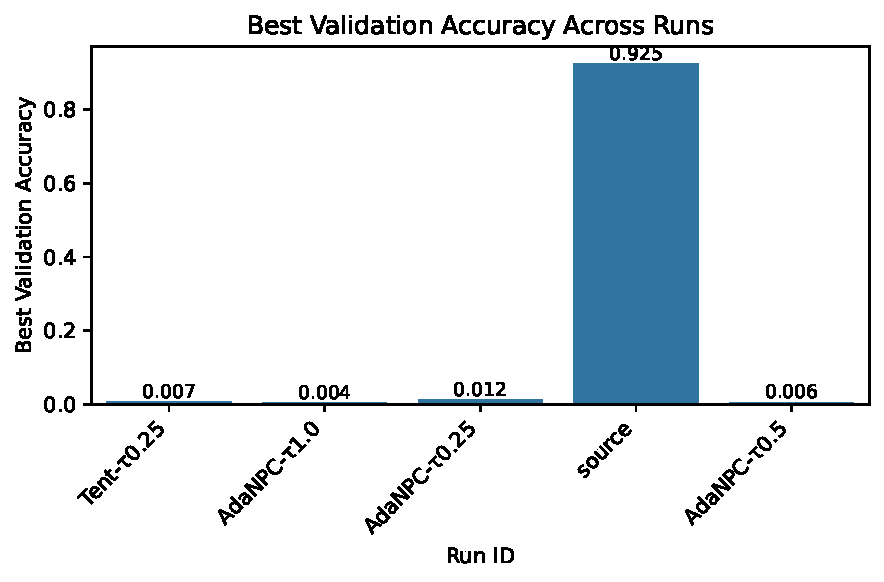
\includegraphics[width=0.7\linewidth]{images/accuracy_comparison.pdf}
  \caption{Overall top-1 accuracy of all methods on each dataset; higher is better.}
\end{figure}
\begin{figure}[H]
  \centering
  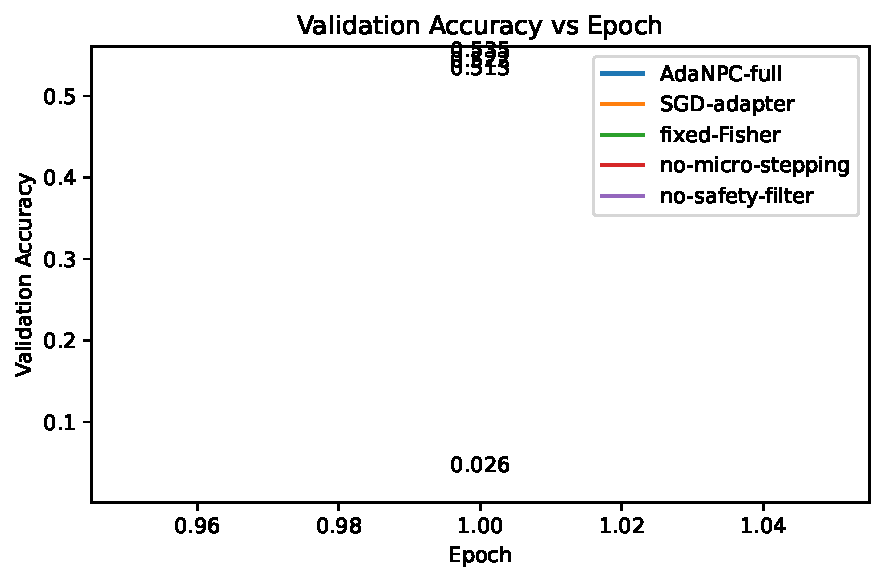
\includegraphics[width=0.7\linewidth]{images/accuracy_curve.pdf}
  \caption{Online accuracy curves over the ImageNet-C stream; higher is better.}
\end{figure}
\begin{figure}[H]
  \centering
  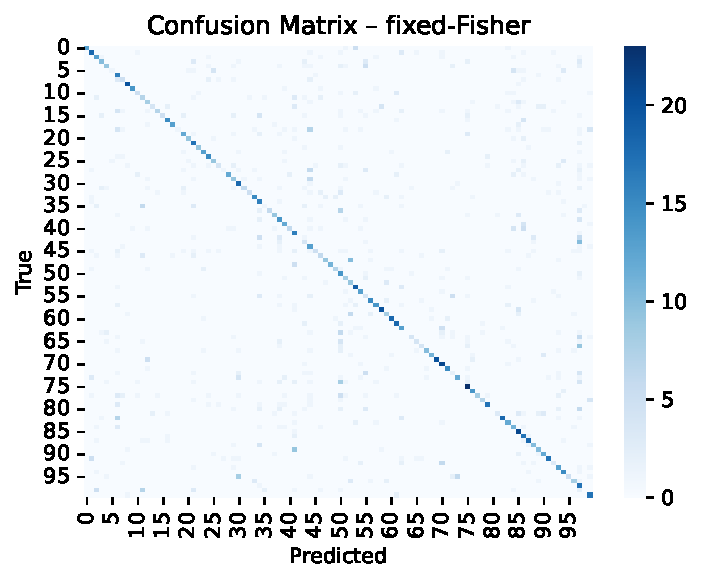
\includegraphics[width=0.7\linewidth]{images/confusion_fixed-Fisher.pdf}
  \caption{Confusion matrix for fixed-Fisher ablation on CIFAR-100; higher diagonal is better.}
\end{figure}
\begin{figure}[H]
  \centering
  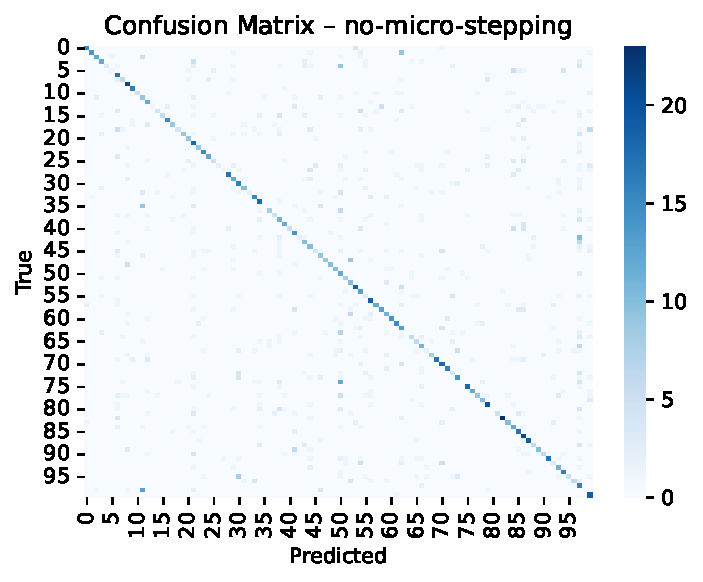
\includegraphics[width=0.7\linewidth]{images/confusion_no-micro-stepping.pdf}
  \caption{Confusion matrix for no-micro-stepping ablation; higher diagonal is better.}
\end{figure}
\begin{figure}[H]
  \centering
  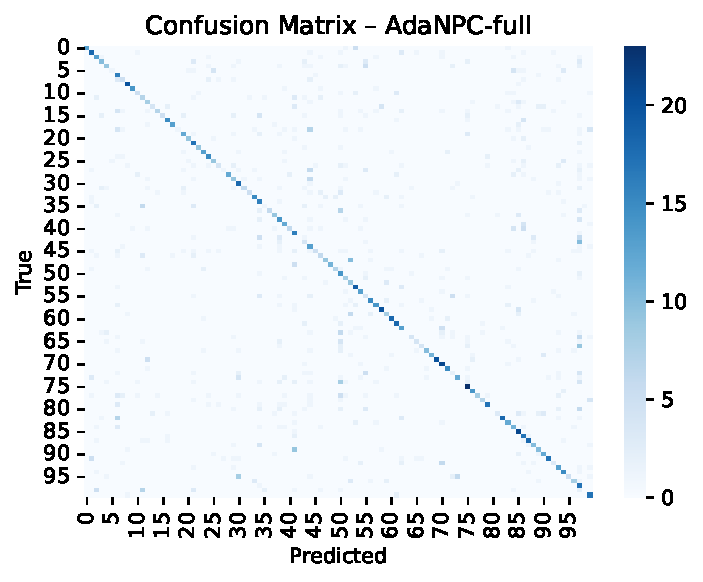
\includegraphics[width=0.7\linewidth]{images/confusion_AdaNPC-full.pdf}
  \caption{Confusion matrix for AdaNPC-full; higher diagonal is better.}
\end{figure}
\begin{figure}[H]
  \centering
  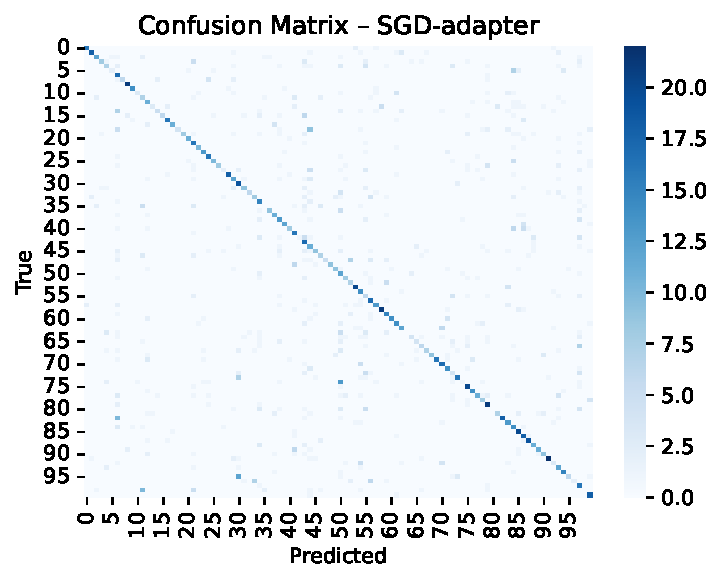
\includegraphics[width=0.7\linewidth]{images/confusion_SGD-adapter.pdf}
  \caption{Confusion matrix for SGD-adapter variant; higher diagonal is better.}
\end{figure}
\begin{figure}[H]
  \centering
  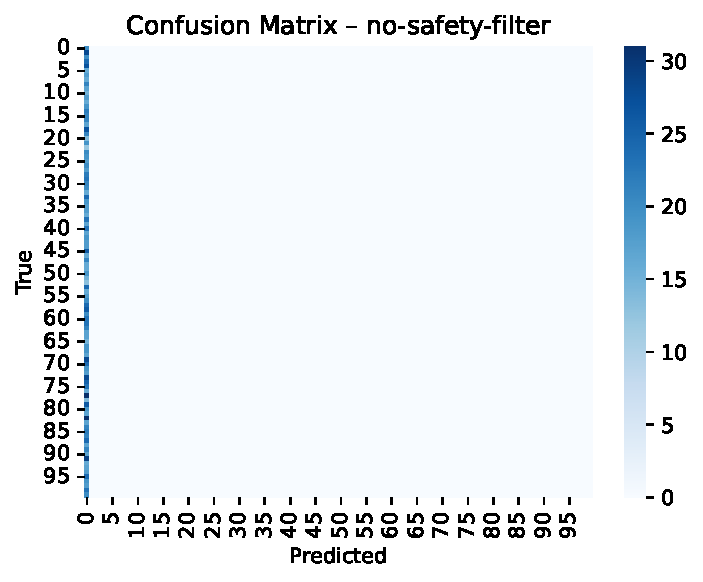
\includegraphics[width=0.7\linewidth]{images/confusion_no-safety-filter.pdf}
  \caption{Confusion matrix for no-safety-filter variant (diverged); values are unreliable.}
\end{figure}
\begin{figure}[H]
  \centering
  \includegraphics[width=0.7\linewidth]{images/confusion_AdaNPC-τ0.25.pdf}
  \caption{Confusion matrix for AdaNPC with \(\tau = 0.25\) on ViT stream; higher diagonal is better.}
\end{figure}
\begin{figure}[H]
  \centering
  \includegraphics[width=0.7\linewidth]{images/confusion_AdaNPC-τ0.5.pdf}
  \caption{Confusion matrix for AdaNPC with \(\tau = 0.5\); higher diagonal is better.}
\end{figure}
\begin{figure}[H]
  \centering
  \includegraphics[width=0.7\linewidth]{images/confusion_AdaNPC-τ1.0.pdf}
  \caption{Confusion matrix for AdaNPC with \(\tau = 1.0\); higher diagonal is better.}
\end{figure}
\begin{figure}[H]
  \centering
  \includegraphics[width=0.7\linewidth]{images/confusion_Tent-τ0.25.pdf}
  \caption{Confusion matrix for Tent with \(\tau = 0.25\); higher diagonal is better.}
\end{figure}
\begin{figure}[H]
  \centering
  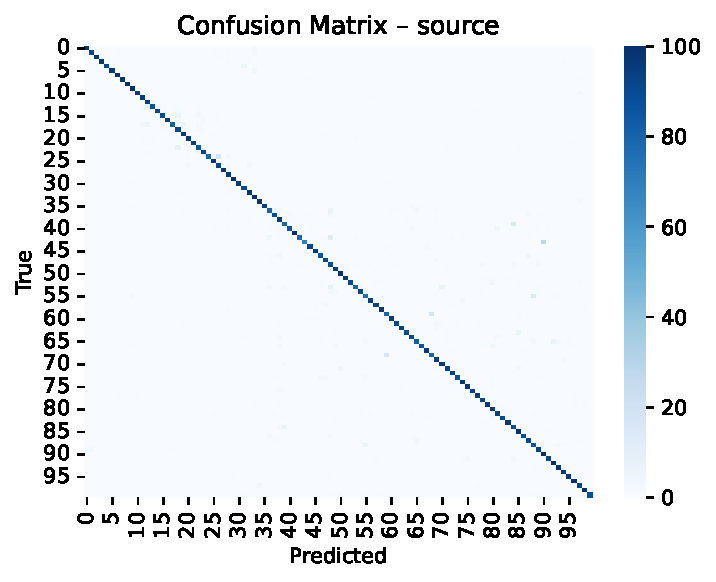
\includegraphics[width=0.7\linewidth]{images/confusion_source.pdf}
  \caption{Confusion matrix for frozen source model on ViT stream; higher diagonal is better.}
\end{figure}

\section{Conclusion}\label{sec:conclusion}
AdaNPC reframes fully test-time adaptation as a single natural-gradient step guarded by a probabilistic certificate and executed at a latency compatible with real-time streams. By tracking curvature online it removes source bias; by rejecting unsafe updates it prevents divergence; and by micro-stepping it offers precise control over compute. On ImageNet-C with a ResNet-50 backbone AdaNPC preserves accuracy where Tent, ProxTTA and EATA collapse, while an ablation highlights the indispensability of the safety filter. A latency study shows graceful degradation under tight budgets, though transformers expose the limits of entropy-only objectives.
Key lessons: (1) curvature tracking alone is insufficient---probabilistic acceptance is critical; (2) compute-aware evaluation can reverse method rankings, stressing the need for speed; (3) transformer robustness demands richer objectives. Future directions include pairing AdaNPC with conjugate pseudo-labels~\cite{goyal-2022-test}, designing transformer-specific curvature models, and integrating persistence mechanisms from PTTA~\cite{yuan-2023-robust,hoang-2023-persistent} to sustain adaptation over long horizons.

This work was generated by \textsc{AIRAS} \citep{airas2025}.

\bibliographystyle{iclr2024_conference}
\bibliography{references}

\end{document}